%%%%%%%%%%%%%%%%%%%%%%%%%%%%%%%%%%%%%%%%%%%%%%%%%%%%%%%%%%%%%%%%%%%%%%%%%%%%%%%%
% \documentclass[12pt,papel,twoside]{ibtesis}
\documentclass[12pt,screen,twoside,pagebackref]{ibtesis}
% \documentclass[12pt,papel,singlespace,oneside]{ibtesis}
% \documentclass[12pt,papel,preprint,singlespace,oneside]{ibtesis}
\usepackage[normalem]{ulem}

%%%%%%%%%%%%%%%%%%%%% Paquetes extra %%%%%%%%%%%%%%%%%%%%%%%%%%%%%%%%%%%%%%%%%%%
% Por conveniencia: aqu\'{\i} puede cargar todos los paquetes y definir los comandos 
% que necesite
\usepackage{ibextra}
\usepackage{physics}
\makeatletter
\setlength{\@fptop}{0pt}
\makeatother
\decimalpoint



%%%%%%%%%%%%%%%%%%%%%%%%%%%%%%%%%%%%%%%%%%%%%%%%%%%%%%%%%%%%%%%%%%%%%%%%%%%%%%%%
%%%%%%%%%%%%%%%%%%%%% Informacion sobre la tesis %%%%%%%%%%%%%%%%%%%%%%%%%%%%%%%
\title{Efecto de repulsi\'{o}n interat\'{o}mica en modos cero de Majorana en un sistema de punto cu\'{a}ntico acoplado a un nanocable superconductor}
\author{Renzo Kenyi Takagui Perez}
\director{Dr. Armando Aligia}
\carrera{Tesis de Maestría en Ciencias Físicas}
\grado{}
\laboratorio{Grupo de Teoría de Materia Condensada - Centro At\'{o}mico Bariloche}
\jurado{Dr. Jorge Facio\\
Dr. Pablo Cornaglia\\
Dr. Alejandro Lobos} 

\palabrasclave{Cadena de Kitaev, Fases Topol\'{o}gicas, Modos cero de Majorana, Superconductores, punto cu\'{a}ntico}
\keywords{microwave resonators, quality factor, SONNET simulations}
% Si queremos poner la fecha manualmente:
% \date{Diciembre de 2099}

%%%%%%%%%%%%%%%%%%%%%%%%%%%%%%%%%%%%%%%%%%%%%%%%%%%%%%%%%%%%%%%%%%%%%%%%%%%%%%%%
%\titlepagefalse % Si no quiere compilar la portada descomente esta linea
%\includeonly{apendices} % Compilar s\'{o}lo estos archivos 
\graphicspath{{figs/}} % Lugar donde encontrar las figuras generales (se puede poner uno en cada cap{\'{\i}}tulo)
%%%%%%%%%%%%%%%%%%%%%%%%%%%%%%%%%%%%%%%%%%%%%%%%%%%%%%%%%%%%%%%%%%%%%%%%%%%%%%%%


\begin{document}

% Dentro del environment 'preliminary' va:
% la dedicatoria, resumen, abstract, indices
\begin{preliminary}
% Escriba su dedicatoria
\agradecimientos{
...
}
%\dedicatoria{
%A mi familia y amigos \sout{(y a chiquito)}\\
%}

%%% \'{I}ndices %%%%



\tableofcontents                %\'{I}ndice


\begin{resumen}%
En el contexto de una configuraci\'{o}n en el que un punto cu\'{a}ntico es usado como una sonda local para estudiar la calidad de modos de Majorana en un nanocable superconductor, investigamos el efecto que tienen sobre estos la introducci\'{o}n de un t\'{e}rmino de respulsi\'{o}n coulombiana entre el punto y el cable cu\'{a}ntico.\\
En modelos previos, el sistema es descrito por hamiltonianos efectivos a bajas energ\'{i}as que, en su mayor\'{i}a, no toman en cuenta un posible efecto de la repulsi\'{o}n coulombiana. Sin embargo, en el estudio realizado por Ricco \emph{et alia}, los autores usan un modelo que incluye dicha repulsi\'{o}n y afirman que la presencia de este t\'{e}rmino arruina la protecci\'{o}n topol\'{o}gica que poseen los modos cero de Majorana (MZMs).\\
En este trabajo de maestr\'{i}a, sostenemos la tesis de que estudiar el sistema a trav\'{e}s de un hamiltoniano efectivo a bajas energ\'{i}as no captura el verdadero efecto de un t\'{e}rmino de repulsi\'{o}n coulombiana en los MZMs. En lugar de un hamiltoniano efectivo, consideramos t\'{e}rminos de m\'{a}s altas energ\'{i}as y modelamos la repulsi\'{o}n como un t\'{e}rmino de interacci\'{o}n entre el punto y el sitio m\'{a}s cercano a este en el nanocable. Seguidamente, obtenemos num\'{e}ricamente valores de expectaci\'{o}n y el perfil de espectro de energ\'{i}as donde notamos que la \'{u}nica situaci\'{o}n donde los MZMs pierden su protecci\'{o}n topol\'{o}gica es cuando tratamos con un nanocable corto y el espectro de energ\'{i}as presenta un patr\'{o}n de diamante.\\
La presente tesis consta de cuatro cap\'{i}tulos. En el cap\'{i}tulo 1, daremos una breve introducci\'{o}n a los modos de Majorana, cadena de Kitaev y el modelo propuesto por Ricco \emph{et alia}. Luego, en el cap\'{i}tulo 2, introducimos un m\'{e}todo anal\'{i}tico que nos permite conocer la forma matricial de los hamiltonianos que estudiamos y analizamos la cadena de Kitaev aislada. Seguidamente, en el cap\'{i}tulo 3, presentamos los resultados del modelo incluyendo el punto cu\'{a}ntico y el \emph{hopping} y la interacci\'{o}n con el primer sitio de la cadena que sostienen la tesis descrita arriba. Finalmente, en el cap\'{i}tulo 4, mencionamos las conclusiones del presente trabajo de investigaci\'{o}n. 
\begin{center}
    Esta maestr\'{i}a est\'{a} basada en el trabajo cient\'{i}fico: 
    \begin{itemize}
        \item \cite{perez2023effect} R. Kenyi Takagui-Perez, A. Aligia. Effect of interatomic repulsion on majorana zero modes in a coupled quantum-dot-superconducting-nanowire hybrid system, arXiv:2309.10888 [cond-mat.mes-hall], enviado a Physical Review B.
    \end{itemize}
\end{center}
\end{resumen}




%%% Local Variables: 
%%% mode: latex
%%% TeX-master: "template"
%%% End: 


\end{preliminary}


% Podemos usar cualquiera de los dos comandos: \input o \include para incluir el texto
%\include{cap1}
%\include{cap2}
%\include{cap2bis}
%\include{cap3}
%
% capitulo Introduccion
%
\chapter{Introducci\'{o}n}

%
% defincion matematica de los Majorana 
%
\section{Definici\'{o}n}
Los llamados modos de Majorana fueron inicialmente planteados por Etore Majorana \cite{Majorana1937TeoriaSD}. Estos los defini\'{o} de tal forma que la part\'{i}cula sea la misma que la antipart\'{i}cula. En t\'{e}rminos de operadores de segunda cuantizaci\'{o}n tienen la propiedad 
\begin{equation}
    \gamma^\dagger=\gamma
\end{equation}
Asimismo, estos obedecen las siguientes reglas de anticonmutaci\'{o}n
\begin{equation}
    \{\gamma_i,\gamma_j\}=2\delta_{ij}
\end{equation}
Todo modo de Majorana puede ser definido en t\'{e}rminos de operadores fermi\'{o}nicos
\begin{equation}
    \gamma=c+c^\dagger
\end{equation}
De igual manera, un modo fermi\'{o}nico ordinario $c^\dagger$ puede ser definido en t\'{e}rminos de dos modos de Majorana como:
\begin{equation}
    c^\dagger=\frac{1}{2}(\gamma_1-i\gamma_2)
\end{equation}

Hasta hora solo hemos hecho una definici\'{o}n matem\'{a}tica pero lo que nos importa es su uso en la f\'{i}sica.

En f\'{i}sica de altas energ\'{i}as los fermiones de Majorana todav\'{i}a no han sido hallados, aunque todav\'{i}a queda por ver si los neutrinos clasifican como estos. En materia condensada, por otra parte, los buscamos como quasipart\'{i}culas. Las b\'{u}squeda de Majoranas se volvi\'{o} una l\'{i}nea de investigaci\'{o}n importante por su posible uso en computaci\'{o}n cu\'{a}ntica. 

Si tenemos una cadena con varios sitios fermi\'{o}nicos numerados $1,...,N$, en modos de Majorana los sitios podr\'{i}an ser escritos como 
\begin{equation}
    \begin{split}
        c_1&=\frac{1}{2}(\gamma_1+i\gamma_2),\quad c^\dagger_1=\frac{1}{2}(\gamma_1-i\gamma_2)\\
        c_2&=\frac{1}{2}(\gamma_3+i\gamma_4),\quad c^\dagger_2=\frac{1}{2}(\gamma_3-i\gamma_4)\\
        &.\\
        &.\\
        &.\\
        c_N&=\frac{1}{2}(\gamma_{2N-1}+i\gamma_{2N}),\quad c^\dagger_2=\frac{1}{2}(\gamma_{2N-1}-i\gamma_{2N})
    \end{split}
\end{equation}
Ya que siempre podemos expresar un fermi\'{o}n como dos modos de Majorana, en principio un Hamiltoniano tambi\'{e}n puede ser enteramente descrito por ellos. Hasta ahora no hemos hecho m\'{a}s que definir los Majorana en relaci\'{o}n con los fermiones pero pronto se les dar\'{a} un significado a un Majorana individual.
%
%
%
\section{Aniones}
Los modos de Majorana no pueden ser identificados ni como fermiones ordinarios ni como bosones, la estad\'{i}stica que presentan u obedecen es diferente. En el caso de las part\'{i}culas indistingibles, que acabamos de mencionar, al ser intercambiadas adquieren o no un cambio de signo en la funci\'{o}n de onda. 
\begin{equation}
\begin{split}    \psi(x_1,x_2)&=+\psi(x_2,x_1)\rightarrow\text{Bosones}\\
    \psi(x_1,x_2)&=-\psi(x_2,x_1)\rightarrow\text{Fermiones}
\end{split}
\end{equation}
Podemos pensar en este cambio de signo como un cambio de fase que la funci\'{o}n de onda adquiere cuando f\'{i}sicamente movemos las part\'{i}culas alrededor una de la otra. Pensar en esto en una sola dimensi\'{o}n puede no tener sentido ya que no habr\'{i}a espacio para el intercambio. Sin embargo, en dos dimensiones se encuentra una nueva forma de pensar en la fase adquirida por las funciones de onda. 

Supongamos que tenemos dos part\'{i}culas id\'{e}nticas en dos dimensiones y las intercambiamos de la forma que hemos descrito, o sea movi\'{e}ndolas una alrededor de la otra. La funci\'{o}n de onda adquirir\'{a} una fase. La forma en c\'{o}mo las moveremos ser\'{a} en sentido antihorario. 
\begin{equation}
    \psi(x_1,x_2)\rightarrow e^{i\theta}\psi(x_1,x_2)
\end{equation}
Si realizamos de nuevo el intercambio en sentido antihorario, la nueva fase no ser\'{a} $+$ o $-$, sino una fase no trivial $e^{i2\theta}$.
\begin{equation}
    \psi(x_1,x_2)\rightarrow e^{i2\theta}\psi(x_1,x_2)
\end{equation}
El caso especial de $\theta=0,\pi$ pertenece al de los bosones y fermiones, respectivamente. Esto quiere decir que existe todo un espectro de estad\'{i}sticas $\theta$ y cuyas part\'{i}culas que la obedecen las llamaremos \emph{aniones}. Esta estad\'{i}stica tambi\'{e}n es llamada \emph{estad\'{i}stica fraccionaria}. La idea de los aniones fue explorada primero por Frank Wikczek\cite{PhysRevLett49957}\cite{RevModPhys801083}.\\
A partir de estas ideas se puede hablar de operaciones de trenzado (\emph{braiding operations}) en las que una operaci\'{o}n del grupo de trenzas (\emph{braid group}) puede ser visualizado como un conjunto de trayectorias de las part\'{i}culas en la dimensi\'{o}n $2+1$ espacio-tiempo en el que las dos part\'{i}culas se cruzan pero de tal forma que podamos diferenciar el camino que tom\'{o} cada una.
Por ejemplo $\sigma_1$ y $\sigma_2$ vendr\'{i}an a ser estas operaciones del grupo de trenzado tal que las part\'{i}culas afectadas tendr\'{a}n que seguir las trayectorias como en la figura\ref{fig:braiding}. El saber qu\'{e} trayectoria est\'{a} por encima de otra es importante porque no es lo mismo aplicar $\sigma_1\sigma_2$ que $\sigma_2\sigma_1$, es decir el grupo de trenzado es un \emph{grupo no-abeliano}. 
%
% Operaciones de Braiding
%
\begin{figure}[H]
    \centering
    \includegraphics[width=0.80\textwidth]{ch1f/braiding.png}
    \caption{Aplicaci\'{o}n de operaciones de trenzado. En todos los casos presentes se consideran tres part\'{i}culas las cuales poseen trayectorias que las vamos a ir modificando dependiendo de qu\'{e} operaci\'{o}n de trenzado aplicamos. Si las posiciones en las que terminan las part\'{i}culas son las mismas en las que empezaron sin importar las operaciones que se aplicaron entonces estas ser\'{a}n equivalentes.}
    \label{fig:braiding}
\end{figure}
La raz\'{o}n porque nos interesan los modos de Majorana y la estad\'{i}stica no-abeliana dada es porque una forma de atacar el problema de las computadoras cu\'{a}nticas tolerantes a fallos \cite{KITAEV20032}\cite{Bravyi2000FermionicQC} es embeber informaci\'{o}n de forma robusta en fermiones no locales, los cuales pueden encontrarse como quasipart\'{i}culas con el comportamiento de aniones, m\'{a}s espec\'{i}ficamente Majoranas.\\
Ahora imaginemos que tenemos a cuatro Majoranas en un cable unidimensional, si quisieramos intercambiarlos de posici\'{o}n inevitablemente estos se encontrar\'{i}an y colisionan, por esta raz\'{o}n la estad\'{i}stica no est\'{a} bien definida para esta dimension. Para realizar operaciones con fermiones de Majorana necesitamos tenerlos siempre distanciados y es ah\'{i} donde entra el concepto de \emph{braiding}, que pict\'{o}ricamente se puede ver como una uni\'{o}n o empalme al superconductor unidimensional donde podemos guardar a un Majorana (rojo) como en la figura \ref{fig:braiding1} y podemos ahora pasar el Majorana (azul) de la derecha a la izquierda, y, asimismo pasar el Majorana guardado (rojo) a la derecha como en la figura \ref{fig:braiding2}. En mec\'{a}nica cu\'{a}ntica operaciones como estas usualmente se escriben como una transformaci\'{o}n $\ket\Psi\rightarrow U\ket\Psi$, en el caso de fermiones o bosones el $U$ es una constante $+1$ o $-1$ seg\'{u}n corresponde. Bajo las condiciones que nos imponen los Majoranas es enteramente posible que $U$ sea otra cosa que $\pm 1$, sino que puede llegar a ser una matriz de rotati\'{o}n que aplicamos a la funci\'{o}n de onda. Si tenemos varias operaciones de \emph{braiding} o simplemente intercambio significa que aplicaremos varias rotaciones, es decir, multiplicaci\'{o}n de matrices y estas operaciones pueden ser no-conmutativas.
\begin{figure}[ht]
\centering
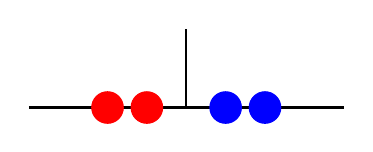
\begin{tikzpicture}
    % Horizontal line
    \draw[thick] (0,0) -- (4,0);
    % Vertical line in the middle (T shape)
    \draw[thick] (2,0) -- (2,1);
    % Red balls on the left
    \filldraw [red] (1,0) circle (0.2);
    \filldraw [red] (1.5,0) circle (0.2);
    % Blue balls on the right
    \filldraw [blue] (2.5,0) circle (0.2);
    \filldraw [blue] (3,0) circle (0.2);
\end{tikzpicture}
\caption{Se tiene la esperanza de que con los modos de Majorana ser\'{a} posible hacer operaciones l\'{o}gicas con qubits, este dibujo rudimentariamente presenta una operaci\'{o}n simple que es la de intercambiar de lugar a dos Majoranas.}
\label{fig:braiding1}
\end{figure}

\begin{figure}[ht]
\centering
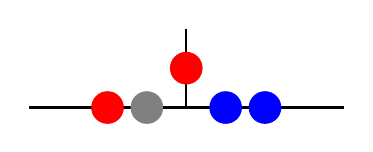
\begin{tikzpicture}
    % Horizontal line
    \draw[thick] (0,0) -- (4,0);
    % Vertical line in the middle (T shape)
    \draw[thick] (2,0) -- (2,1);
    % Red ball on the vertical line
    \filldraw [red] (2,0.5) circle (0.2);
    % Other red ball on the left
    \filldraw [red] (1,0) circle (0.2);
    \filldraw [gray] (1.5,0) circle (0.2);
    % Blue balls on the right
    \filldraw [blue] (2.5,0) circle (0.2);
    \filldraw [blue] (3,0) circle (0.2);
\end{tikzpicture}
\caption{Ya que tener cable unidimensional no permitir\'{i}a el intercambio, si hacemos un acople al cable con alguna otra juntura donde podamos almacenar momentaneamente a uno de los Majorana entonces ah\'{i} s\'{i} es posible llevar a cabo la operaci\'{o}n.}
\label{fig:braiding2}
\end{figure}
La raz\'{o}n porque nos interesan los modos de Majorana y la estad\'{i}stica no-abeliana dada es porque una forma de atacar el problema de las computadoras cu\'{a}nticas tolerantes a fallos \cite{KITAEV20032}\cite{Bravyi2000FermionicQC} es embeber informaci\'{o}n de forma robusta en fermiones no locales, los cuales pueden encontrarse como quasipart\'{i}culas con el comportamiento de aniones, m\'{a}s espec\'{i}ficamente Majoranas. Una vez que tenemos Majoranas queremos realizar operaciones sobre qubits, pero, como hemos visto, esto se puede lograr usando operaciones de trenzado.\\
Por otro lado, hablar de aniones no solo nos limita al campo de materia condensada. El tema nos conecta directamente con el estudio de computaci\'{o}n cu\'{a}ntica topol\'{o}gica \cite{freedman2000} y teor\'{i}a cu\'{a}ntica de campos topol\'{o}gica \cite{lancaster2014quantum}\cite{ZeeQuantum} que, otra vez, nos vuelve a conectar con temas de materia condensada como por ejemplo: el estudio de v\'{o}rtices, el efecto Aharonov-Bohm o la teor\'{i}a de Chern-Simons \cite{Witten}.\\
Desde el 2021, luego de bastantes a\~{n}os de resultados parciales en la b\'{u}squeda de Majoranas, combinando t\'{e}cnicas te\'{o}ricas y experimentales de BEC (condensado de Bose-Einstein) y BCS (teor\'{i}a de superconductividad de Bardeen–Cooper–Schrieffer) \cite{anyonsandmajo} hay mucha promesa en por fin poder identificar aniones, en particular Majoranas.
\section{Introducci\'{o}n a la cadena de Kitaev}
Debido a su relevancia para nuestros resultados novedosos con la cadena de Kitaev interactuando con un punto cu\'{a}ntico, repasamos brevemente la cadena aislada.

En resumen, el paper de Kitaev \cite{YKitaev_2001} nos cuenta que en un sistema fermi\'{o}nico sin esp\'{i}n con una brecha en el espectro del volumen posee estados de borde que pueden ser descritos por fermiones de Majorana, que podr\'{i}an ser de utilidad como qubits por ser robustos ante perturbaciones.

El sistema fermi\'{o}nico que nos plantea Kitaev es el de una cadena unidimensional en el r\'{e}gimen sin esp\'{i}n (esto se podr\'{i}a lograr aplicando un campo magn\'{e}tico), superconductor (por superconductividad inducida por proximidad) en el que exista una brecha en el espectro. Con esta receta podemos empezar planteando el Hamiltoniano del sistema
\begin{equation}
      H=\sum_j [ -\mu (c_j^\dagger c_j - \frac{1}{2})-t(c_j^\dagger c_{j+1}+c_{j+1}^\dagger c_j) + (\Delta c_j c_{j+1}+\Delta^* c_{j+1}^\dagger c^\dagger_j)]
      \label{hammy_kitaev}
\end{equation}
donde el primer t\'{e}rmino es la energ\'{i}a de ocupaci\'{o}n por sitio, el segundo es el t\'{e}rmino de salto y el \'{u}ltimo t\'{e}rmino es la creaci\'{o}n o destrucci\'{o}n de pares de Cooper. A este modelo lo llamamos \emph{cadena de Kitaev}, o m\'{a}s especificamente, a la cadena que presenta modos cero de Majorana. 
Para la discusi\'{o}n de la siguiente secci\'{o}n escribimos cada operador fermi\'{o}nico que aparece en la ecuaci\'{o}n (\ref{hammy_kitaev}) como combinaci\'{o}n lineal de dos fermiones de Majorana.
\begin{equation}
    c_j^\dagger=\frac{1}{2}(\gamma_{2j-1}-i\gamma_{2j}),\quad c_j=\frac{1}{2}(\gamma_{2j-1}+i\gamma_{2j}) 
\end{equation}
donde $j$ ennumera el sitio de la cadena unidimensional.
%
% Fase topologica y trivial de la cadena 
%
\section{Fase topol\'{o}gica y trivial de la cadena}
A modo de explorar algunas de las propiedades de la cadena de Kitaev consideramos dos casos simples para cada fase:\\
(i) Fase trivial. Caso cuando $\mu\neq 0$ y $t=\Delta=0$. Solo para fines de ver c\'{o}mo se combinan los Majoranas en este caso, reemplazamos los operadores originales por su equivalente en t\'{e}rminos de Majorana.
    \begin{equation}
            H=-\mu\sum_{n=1}^N (c^\dagger_n c_n-\frac{1}{2})=\frac{i}{2}(-\mu) \sum_{n=1}^N \gamma_{2n-1}\gamma_{2n}
    \end{equation}
    %
    % Figura 
    %
    \begin{center}
    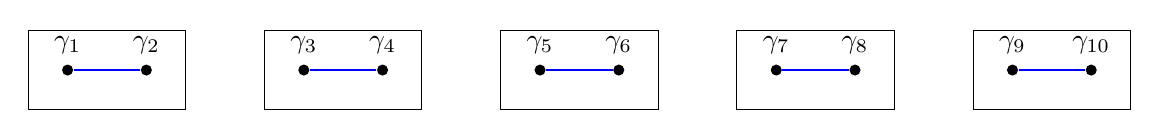
\begin{tikzpicture}[site/.style={rectangle, draw, minimum size=1cm, minimum width=2cm}]
    
    % Intra-cell pairing
    \foreach \i in {1,...,5} {
        % Calculate the labels for c
        \pgfmathtruncatemacro{\labelone}{2*\i-1}
        \pgfmathtruncatemacro{\labeltwo}{2*\i}
    
        % Draw the site
        \node[site] (site\i) at (3*\i-3,0) {};
    
        % Draw Majorana operators and labels
        \node[circle,fill=black,inner sep=0pt,minimum size=4pt,label=above:\( \gamma_{\labelone} \)] (c\labelone) at ([xshift=-0.5cm]site\i.center) {};
        \node[circle,fill=black,inner sep=0pt,minimum size=4pt,label=above:\( \gamma_{\labeltwo} \)] (c\labeltwo) at ([xshift=0.5cm]site\i.center) {};
    
        % Draw the pairing line
        \draw[thick, blue] (c\labelone) -- (c\labeltwo);
    }
    \end{tikzpicture}
    \end{center}
    los Majoranas se acoplan con los del mismo sitio. Entonces, en la fase trivial no pasa nada interesante. El estado fundamental estar\'{a} todo lleno o todo vac\'{i}o dependiendo del $\mu$, y el espectro no contiene estados de energ\'{i}a nulo.\\
(ii) Fase topol\'{o}gica. $\mu=0$ y $t=\Delta\neq 0$. Volvemos a reemplazar todos los operadores fermi\'{o}nicos por Majoranas y vemos qu\'{e} pasa
    \begin{equation}
        \begin{split}
            H&=\sum_{n=1}^N -t(c_n^\dagger c_{n+1}+c_{n+1}^\dagger c_n) + \Delta c_n c_{n+1}+\Delta^*c^\dagger_{n+1}c_n^\dagger\\
            &=\sum_{n=1}^N-\frac{t}{4}\Big[(\gamma_{2n-1}-i\gamma_{2n})(\gamma_{2n+1}+i\gamma_{2n+2})+(\gamma_{2n+1}-i\gamma_{2n+2})(\gamma_{2n-1}+i\gamma_{2n})\Big]\\
            &+\frac{\Delta}{4} (\gamma_{2n-1}+i\gamma_{2n})(\gamma_{2n+1}+i\gamma_{2n+2})+\frac{\Delta^*}{4}(\gamma_{2n+1}-i\gamma_{2n+2})(\gamma_{2n-1}-i\gamma_{2n})\\
            &=\frac{1}{4}\sum_{n=1}^N -t\Big[ \gamma_{2n-1}\gamma_{2n+1}+i\gamma_{2n-1}\gamma_{2n+2}+i\gamma_{2n}\gamma_{2n+1}\\    &+\gamma_{2n}\gamma_{2n+2}+\gamma_{2n+1}\gamma_{2n-1}+i\gamma_{2n+1}\gamma_{2n}-i\gamma_{2n+2}\gamma_{2n-1}+\gamma_{2n+2}\gamma_{2n} \Big]\\
            &+\frac{\Delta}{4}\Big[ \gamma_{2n-1}\gamma_{2n+1}+i\gamma_{2n-1}\gamma_{2n+2}+i\gamma_{2n}\gamma_{2n+1}-\gamma_{2n}\gamma_{2n+2}\\
            &+\gamma_{2n+1}\gamma_{2n-1}-i\gamma_{2n+1}\gamma_{2n}-i\gamma_{2n+2}\gamma_{2n-1}-\gamma_{2n+2}\gamma_{2n}\Big]\\
            &=\frac{t}{4}\sum_n[-2i\gamma_{2n-1}\gamma_{2n+2}+2i\gamma_{2n}\gamma_{2n+1}+2i\gamma_{2n-1}\gamma_{2n+2}+2i\gamma_{2n}\gamma_{2n+1}]\\
            &=t\sum_n i\gamma_{2n}\gamma_{2n+1}
        \end{split}
    \end{equation}
        %
    % Figura
    %
    \begin{center}
        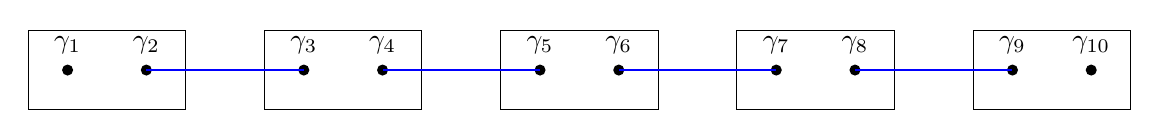
\begin{tikzpicture}[site/.style={rectangle, draw, minimum size=1cm, minimum width=2cm}]

    % Draw sites and Majorana fermions
    \foreach \i in {1,...,5} {
        % Calculate the labels for c
        \pgfmathtruncatemacro{\labelone}{2*\i-1}
        \pgfmathtruncatemacro{\labeltwo}{2*\i}
    
        % Draw the site
        \node[site] (site\i) at (3*\i-3,0) {};
    
        % Draw Majorana operators and labels
        \node[circle,fill=black,inner sep=0pt,minimum size=4pt,label=above:\( \gamma_{\labelone} \)] (c\labelone) at ([xshift=-0.5cm]site\i.center) {};
        \node[circle,fill=black,inner sep=0pt,minimum size=4pt,label=above:\( \gamma_{\labeltwo} \)] (c\labeltwo) at ([xshift=0.5cm]site\i.center) {};
    }
    
    % Draw the inter-cell pairing lines as solid lines connecting the rightmost Majorana of one site to the leftmost Majorana of the next
    \foreach \i [evaluate=\i as \nexti using int(\i+1)] in {1,...,4} {
        \pgfmathtruncatemacro{\labeltwo}{2*\i}
        \pgfmathtruncatemacro{\labelthree}{2*\i+1}
        \draw[thick, blue] ([xshift=0.5cm]site\i.center) -- ([xshift=-0.5cm]site\nexti.center);
    }
    \end{tikzpicture}
    \end{center}
    En este caso vemos que ahora los Majoranas tipo 2 de un sitio se acoplan con los de tipo 1 pero del sitio siguiente. Este acoplamiento da lugar a que los operadores de Majorana de los bordes no aparezcan en el Hamiltoniano. Por lo tanto, ambos tendr\'{i}an energ\'{i}a degenerada en cero. Adem\'{a}s, gracias a esto tenemos dos estados fundamentales degenerados ortogonales entre s\'{i}. Para ver esto definimos nuevos operadores fermi\'{o}nicos pero conformados por estos Majoranas acoplados
    \begin{equation}
        \tilde c^\dagger_j=(\gamma_{2j}-i\gamma_{2j+1})/2,\quad \tilde c_j = (\gamma_{2j}+i\gamma_{2j+1})/2
    \end{equation}
    \begin{equation}
        \gamma_{2j}=\tilde c_j^\dagger+\tilde c_j,\quad \gamma_{2j+1}=\frac{\tilde c_j^\dagger-\tilde c_j}{i}
    \end{equation}
    reemplazando en el Hamiltoniano este se convierte en
    \begin{equation}
        \begin{split}
            H&=it\sum_{n=1}^{N-1}\gamma_{2n}\gamma_{2n+1}\\
            &=it\sum_{n=1}^{N-1}\Big(\tilde c^\dagger_j - \tilde c_j \Big)\Big(\frac{\tilde c^\dagger_j + \tilde c_j}{i} \Big)\\
            &=t\sum_{n=1}^{N-1} \tilde{c_j}^\dagger\tilde{c_j}^\dagger+ \tilde{c_j}^\dagger\tilde{c_j}- \tilde c_j \tilde{c_j}^\dagger-\tilde c_j \tilde c_j\\
            &=2t\sum_{n=1}^{N-1}\Big(\tilde c_j^\dagger \tilde c_j - \frac{1}{2}\Big)
        \end{split}
        \label{hammy_kitaev_topo}
    \end{equation}
Teniendo estos dos casos a la mano podemos conjeturar que existen dos fases bien diferenciadas en el sistema dependiendo de los valores de los par\'{a}metros. Al primer caso lo llamamos el caso trivial ya que no est\'{a} pasando nada interesante y el rol de los Majorana no importa mucho. Sin embargo, en el segundo caso vemos c\'{o}mo la presencia de los Majorana de los bordes constituyen un fermi\'{o}n de Dirac deslocalizado de energ\'{i}a cero en medio del gap. Esta fase, donde hay estados con energ\'{i}as muy cercanas a cero en medio del gap, ser\'{a} llamada \emph{fase topol\'{o}gica}.
%
%
%
\section{Modelo previo de un punto cu\'{a}ntico acoplado a un cable superconductor topol\'{o}gico}
Ahora introduciremos el modelo base con el que se trabaja en la tesis: un punto cu\'{a}ntico acoplado a uno de los extremos de un nanocable. El porqu\'{e} resulta este modelo interesante es que se puede usar el punto cu\'{a}ntico como una prueba local para realizar espectroscop\'{i}a de Majoranas en un nanocable supercondutor. Esta configuraci\'{o}n nos va a permitir disernir si los modos cero que se observan en los experimentos de anomal\'{i}as de pico cero son de origen topol\'{o}gico o si se trata de alg\'{u}n otro fen\'{o}meno f\'{i}sico. Los primeros en proponer este sistema fueron Prada \emph{et alia} \cite{PhysRevB.96.085418}. En su investigaci\'{o}n usan un hamiltoniano efectivo a bajas energ\'{i}as y presentan una serie de simulaciones del perfil de espectro de energ\'{i}as donde dependiendo si se trata de un cable corto ($\approx 400$ nm) o cable largo ($\approx 2$ $\mu$m) se puede apreciar o bien diferentes patrones que forman los MZMs, como de  mo\~{n}o o diamante, o una protecci\'{o}n topol\'{o}gica muy robusta incluso si las energ\'{i}as de los autoestados correspondientes al punto cu\'{a}ntico se acercan mucho al cero, pero no tanto como para cruzarse con los MZMs. Luego, Clarke \cite{PhysRevB.96.201109}, extiende estos estudios para medir la calidad o grado de qu\'{e} tan topol\'{o}gico es un sistema de las mismas caracter\'{i}sticas que el modelo de Prada \emph{et alia}. Finalmente, Ricco \emph{et alia} \cite{PhysRevB.102.165104} hacen una extensi\'{o}n m\'{a}s a este modelo incluyendo un t\'{e}rmino de repulsi\'{o}n coulombiana afirmando que este induce una hibridaci\'{o}n adicional en los MZMs. Algunos estudios experimentales que le dan soporte a todos estos trabajos pueden ser le\'{i}dos en las referencias \cite{PhysRevB.98.085125} y \cite{DEEENG}. 
%
% Estudios de Prada et al
%
\begin{comment}
\subsection{Estudio de Prada et al.}
Uno de los mayores problemas a resolver es disernir de manera correcta si en experimentos de transporte que reportan una anomalía \emph{zero-bias}, se trata realmente de Majoranas de origen topológico o si se puede explicar por otros mecanismos.
\begin{figure}[h]
    \centering
    \includegraphics[width=0.7\textwidth]{ch2f/prada1.png}
    \caption{Configuraci\'{o}n del sistema de punto cu\'{a}ntico acoplado a un nanocable.}
    \label{fig:prada_model}
\end{figure}

En el trabajo de Prada \emph{et alia} \cite{PhysRevB.96.085418}, la configuraci\'{o}n con la que trabajan es la de tener nanocables semiconductores con superconductividad inducida por proximidad. Los autores proponen atacar el problema de detectar la calidad de los Majoranas a trav\'{e}s de una sonda local, en este caso un punto cu\'{a}ntico. Su modelo es el de tener a este en uno de los extremos del nanocable, el potencial qu\'{i}mico ser\'{a} controlado por la fuente (\emph{source}) y sumidero (\emph{drain}), la ocupaci\'{o}n del punto cu\'{a}ntico controlado por los potenciales de compuerta (\emph{gate}), e imponiendo acoplamientos $t_{L(R)}$ entre el punto cu\'{a}ntico con los Majoranas ubicados en los extremos del nanocable que llamaremos $\gamma_{L(R)}$ a izquierda y derecha, y, finalmente, incluyen un acoplamiento $\delta$ entre los Majorana tal como se ve en la figura \ref{fig:prada_model}.

Prada et alia usaron un modelo \emph{tight-binding} microsc\'{o}pico en el que corrieron simulaciones para el estudio de hibridaci\'{o}n de modos cero de Majoranas en un cable y estados de \emph{subgap} del punto cu\'{a}ntico. Su Hamiltoniano completo es
\begin{equation}
\begin{split}
H & = H_d + H_w + H_{hop}, \\
H_d & = d^{\dagger}_{\sigma'}(\epsilon_{0}\sigma_0 + B\sigma_z)d_{\sigma} + U n_{\uparrow}n_{\downarrow}, \\
H_w & = \int_{0}^{L_w} dx\text{ }c^{\dagger}_{x\sigma} \left( \frac{\hbar^2 k_x^2}{2m} - \mu \sigma_0 + \alpha k_x \sigma_y + B_0 \sigma_z \right) c_{x\sigma} \\
    & \quad + \Delta (c_{x\uparrow}c_{x\downarrow} + c^{\dagger}_{x\downarrow}c^{\dagger}_{x\uparrow}), \\
H_{hop} & = t(c^{\dagger}_{0\sigma}d_{\sigma} + d^{\dagger}_{\sigma}c_{0\sigma}),
\end{split}
\label{hammy_prada}
\end{equation}
donde $\epsilon_0$ es el nivel de energ\'{i}a del punto, $U$ es la energ\'{i}a de carga, $m$ es la masa efectiva del nanocable, $\alpha$ es el acoplamiento spin-orbita de Rashba, $\Delta$ es el apareamiento superconductor inducido, $\mu$ es el potencial qu\'{i}mico del cable, y $B$ es el desdoblamiento Zeeman original por un campo magn\'{e}tico externo. Para un $B>B_c\equiv \sqrt{\mu^2+\Delta^2}$ el nanocable entra en una fase topol\'{o}gica con estados de Majorana en cada extremo. 
\par Este es un modelo bastante general bajo ciertas reestricciones. El t\'{e}rmino de repulsi\'{o}n es local en el punto cu\'{a}ntico pero no incluye interacci\'{o}n con la cadena. El t\'{e}rmino $Un_\uparrow n_\downarrow$ lo tratan en campo medio. Por otro lado, en palabras de los autores, utilizaron el modelado m\'{a}s simple para el contacto entre el punto y la cadena dando lugar a la parte de su Hamiltoniano $H_{hop}$ que describe un posible salto entre electrones del punto y el primer sitio de la cadena con el mismo esp\'{i}n. Se\~{n}alan que una manera m\'{a}s realista de modelar lo que pasa entre entre los dos dispositivos es considerar dos segmentos del cable, simular una cierta barrera de potencial dada por una compuerta ubicada justo en la juntura donde ambos dispositivos se unen. Indican que en su modelo de \emph{tight-binding} toman una relaci\'{o}n de $1$ a $10$ entre el coeficiente de salto entre el punto cu\'{a}ntico con el extremo izquierdo de la cadena (ver figura \ref{fig:prada_model}) y el coeficiente de salto entre posiciones cercanas en la cadena. En esta tesis se sigue de manera similar tal relaci\'{o}n.
%
% Imagenes Prada y Aguado
% 
\begin{figure}[h]
    \centering
    \includegraphics[width=0.49\linewidth]{ch3f/prada1.png} 
    \caption{(a) y (c) presentan el perfil del espectro de energ\'{i}as para cuando se deja fijo un $\epsilon_0$ y se var\'{i}a el campo magn\'{e}tico. (b) y (d) presentan tambi\'{e}n espectros de energ\'{i}a pero dejando fijo $B$ y variando el nivel de energ\'{i}a del punto cu\'{a}ntico.\cite{PhysRevB.96.085418}. El tama\~{n}o del cable utilizado para sus simulaciones tiene $L_\omega=2$ $\mu$m}
    \label{fig:pradaa1}
\end{figure}

\begin{figure}[h]
    \centering
    \includegraphics[width=0.49\linewidth]{ch3f/prada2.png} 
    \caption{Espectro de energ\'{i}as para una cadena corta de longitud $L_\omega=400$ nm. (a) presenta las energ\'{i}as del sistema segun se var\'{i}a el campo magn\'{e}tico $B$, y (b) y (c) para cuando se var\'{i}a $\epsilon_0$.\cite{PhysRevB.96.085418}.}
    \label{fig:pradaa2}
\end{figure}


La fenomenolog\'{i}a de su modelo de \emph{tight-binding} es mostrada en un perfil del espectro de energ\'{i}a. En la figura \ref{fig:pradaa1}(a) y \ref{fig:pradaa1}(b) se pueden diferenciar clarmente dos fases. En la fase trivial $B<B_c$ solo los niveles del punto cu\'{a}ntico aparecen por debajo de la brecha de energ\'{i}a del superconductor. Para sus simulaciones variando el $B$, Prada \emph{et alia} consideran un nanocable de longitud $L_\omega=2$ $\mu$m con los siguientes par\'{a}metros: $\mu=0$, $\delta=0.5$ meV y un nivel energ\'{e}tico fijo del punto $\epsilon_0\approx 0.25$ meV. Para un $B>B_c$ el nanocable se encontrar\'{a} en la fase topol\'{o}gica donde podremos encontrar MZMs. Para la figura \ref{fig:pradaa2}(c) se usa un $\epsilon_0=1.0$ meV. Por otro lado, en la figura \ref{fig:pradaa2} se lidia con un nanocable corto de $\L_\omega=400$ nm. Para cables suficientemente cortos muestran que habr\'{a} una hibridizaci\'{o}n de los Majoranas que lleva a un comportamiento oscilatorio de los estados que los describen tal como vemos en la figura \ref{fig:pradaa2}(a). Cuando dejan fijo $B$ y empiezan a variar $\epsilon_0$ se observan estas mismas oscilaciones pero adoptando patrones como de mo\~{n}o o de diamante, ver figura \ref{fig:pradaa2}(b) y\ref{fig:pradaa2}(c).
\par Tambi\'{e}n ofrecen una derivaci\'{o}n de su modelo efectivo a bajas energ\'{i}as. En el trabajo original de Kitaev, este ya mencionaba que para cadenas de longitud $L$ finita habr\'{a} una interacci\'{o}n d\'{e}bil entre los dos modos cero de Majorana $\gamma_L$ y $\gamma_R$, donde $\gamma_L$ est\'{a} en el final izquierdo de la cadena y $\gamma_R$ en el final derecho. El hamiltoniano efectivo con el que Kitaev termina tiene la forma de
\begin{equation}
    H_{eff}=\frac{i}{2}t\gamma_L\gamma_R, t\propto e^{-L/l_0}.
\end{equation}
\end{comment}
%
% Estudios de ricco et al.-
%
\subsection{Estudio de Ricco \emph{et alia}}
Para esta tesis resulta importante repasar en cierto detalle el modelo planteado por Ricco \emph{et alia} ya que ser\'{a}n sus resultados los cuales compararemos con los nuestros.

El modelo de Ricco \emph{et alia} es un Hamiltoniano efectivo de bajas energ\'{i}as en el que solo est\'{a}n presentes t\'{e}rminos del punto cu\'{a}ntico y los modos fermi\'{o}nicos de Majorana que se encuentran a los extremos de la cadena unidimensional que est\'{a} acoplada en uno de los extremos con el punto cu\'{a}ntico. A esto se le a\~{n}ade el t\'{e}rmino de interacci\'{o}n coulombiana entre ambos dispositivos que, seg\'{u}n los autores, causa que el desdoblamiento de los MZMs aumente y al hacerlo estos pierden su robustez ante posibles perturbaciones. El Hamiltoniano que propusieron luce como 
\begin{equation}
    \mathcal{H}=\epsilon_d d^\dagger d + i\epsilon_M \gamma_L\gamma_R + i\lambda_L(d-d^\dagger)\gamma_L+\lambda_R(d+d^\dagger)\gamma_R + H_U
    \label{hammy_ricco}
\end{equation}
donde $\epsilon_d$ es la energ\'{i}a de ocupaci\'{o}n del punto cu\'{a}ntico, $\epsilon_M$ es una medida de qu\'{e} tanto acoplamiento o hibridizaci\'{o}n espacial existe entre las funciones de onda de los modos de Majorana de la izquierda el de la derecha, $\lambda_{L(R)}$ indica cu\'{a}nto acoplamiento hay entre los Majoranas de la izquierda y derecha respectivamente con el punto cu\'{a}ntico. Finalmente, el \'{u}ltimo t\'{e}rmino de cuenta de la repulsion coulombiana entre el punto cu\'{a}ntico y el fermi\'{o}n delocalizado $f^\dagger=(\gamma_L+\gamma_R)/2$ formado por ambos Majoranas, este posee la siguiente forma, con $n_f=f^\dagger f$
\begin{equation}
    H_U=U n_d n_f = \frac{1}{2}Un_d\Big( i\gamma_R\gamma_L+\frac{1}{2}\Big)
\end{equation}
$n_f$ representar\'{i}a el total de la ocupaci\'{o}n de la cadena a baja energ\'{i}a. $H_U$ se parece bastante a la del segundo t\'{e}rmino de (\ref{hammy_ricco}). Por eso afirman que debido a la repulsi\'{o}n coulombiana habr\'{a} una hibridizaci\'{o}n extra causando as\'{i} un desdoblamiento m\'{a}s grande en el espectro de energ\'{i}as.\\
En las siguientes subsecciones se describir\'{a}n brevemente los casos que los autores estudiaron, estos son el caso no-interactuante y el caso interactuante. Es decir, cuando tomamos o no en cuenta la repulsi\'{o}n coulombiana. Los gr\'{a}ficos que se mostrar\'{a}n acontinuaci\'{o}n son del paper original. La forma en la que calcularon su espectro de energ\'{i}a fue a trav\'{e}s del c\'{a}lculo de densidad de estados del punto cu\'{a}ntico $\rho_d(V)$ que a temperatura cero es proporcional la conductancia diferencial, $dI/dV \propto \rho_d(V)$, con $V$ correspondiendo al voltaje de bias. La densidad espectral resultante se muestra en las figuras \ref{fig:nointer} y \ref{fig:inter}.
Cabe recordar que la tesis de los autores es que debido a la repulsi\'{o}n coulombiana los MZMs perder\'{a}n su condici\'{o}n de estar topol\'{o}gicamente protegidos, y la forma de mostrarlo es a trav\'{e}s de observar qu\'{e} les pasa a estos modos en el espectro de energ\'{i}a. Si los MZMs pierden su robustez se deber\'{i}a apreciar una separaci\'{o}n de energ\'{i}a mayor donde antes no la hab\'{i}a.
%
% Non interacting case 
%
\subsubsection{Caso no interactuante}
Primero veremos el caso no interactuante, es decir, el caso en el que la repulsi\'{o}n coulombiana est\'{a} apagada. En la figura \ref{fig:nointer}(a) para cuando no hay repulsi\'{o}n y adem\'{a}s no hay separaci\'{o}n adicional por el t\'{e}rmino que acompa\~{n}a a $\epsilon_M$, nos encontramos en el caso ideal donde los MZMs est\'{a}n topol\'{o}gicamente protegidos cerca de energ\'{i}a cero. La situaci\'{o}n cambia cuando empezamos a considerar un $\epsilon_M\neq 0$, es decir, tomar en cuenta hibridaci\'{o}n entre los MZMs. Entonces los MZMs se separan en energ\'{i}a y podemos identificar figuras caracteristicas que se ven en otras referencias como la del mo\~{n}o o de diamante. En la figura \ref{fig:nointer}(b) en el caso de $\epsilon_M\gg \lambda_R$ ocurre una forma de mo\~{n}o y el cruce de nieveles en $\epsilon_d=0$. Si en cambio se considera un coeficiente de hibridaci\'{o}n de Majoranas insignificante a comparaci\'{o}n del acoplamiento entre el punto cu\'{a}ntico y el Majorana de la derecha como en la figura \ref{fig:nointer}(c), los autores obtienen una forma de diamante, o sea un desdoblamiento en $\epsilon_d=0$. Finalmente en la figura \ref{fig:nointer}(d), si los coefficientes $\epsilon_d$, $\lambda_R$ y $\lambda_L$ son comparables, se obtiene un espectro asim\'{e}trico con respecto al eje de energ\'{i}as y ocurre un desplazamiento del cruce hacia la derecha.   
%
%Inicio de Figura no interactuante
\begin{figure}[t]
    \centering
    \includegraphics[width=0.75\textwidth]{ch3f/No interactuante.png}
    \caption{Autoenergías en función de la energía del punto cuántico $\epsilon_d$ para cuando el t\'{e}rmino de repulsi\'{o}n $H_U=0$ en (\ref{hammy_ricco}).}
    \label{fig:nointer}
\end{figure}
%
% Interacting case 
%
\subsubsection{Caso interactuante}
El caso interactuante consiste en tomar en cuenta el t\'{e}rmino de repulsi\'{o}n coulombiana $Un_dn_f$, que, como se explic\'{o} anteriormente, posee una forma muy parecida a la del t\'{e}rmino de hibridaci\'{o}n de los Majorana $\epsilon_M\gamma_L\gamma_R$. Bajo este modelo y consideraciones, sus simulaciones dan que incluso en el caso $\epsilon_M=0$, como en la figura \ref{fig:inter}(a), existe una separaci\'{o}n de energ\'{i}as de los MZMs significando la p\'{e}rdida de protecci\'{o}n top\'{o}logica.

Comparando los paneles de la figura \ref{fig:inter} con los respectivos de la figura \ref{fig:nointer}, vemos que el efecto de la interacci\'{o}n $H_U$ es siempre aumentar el desdoblamiento del caso no interactuante.
%
%Inicio de figura Interactuante
\begin{figure}[t]
    \centering
    \includegraphics[width=0.74\textwidth]{ch3f/interactuante.png}
    \caption{Autoenergías en función de la energía del punto cuántico $\epsilon_d$ para cuando el t\'{e}rmino de repulsi\'{o}n $H_U\neq 0$ en (\ref{hammy_ricco}).}
    \label{fig:inter}
\end{figure}
\chapter{Espectro de energ\'{i}as de la cadena de Kitaev}
Antes de abordar el sistema completo, incluyendo el punto cu\'{a}ntico, estudiamos la cadena de Kitaev finita. Si bien esta se conoce, para ver el efecto de la interacci\'{o}n con el punto cu\'{a}ntico necesitamos informaci\'{o}n detallada de la cadena aislada.\\
Para estudiar el espectro de energ\'{i}as de una cadena aislada finita y extensiones del modelo, introduciremos un m\'{e}todo de mapeo similar a la notaci\'{o}n de Nambu que nos permitir\'{a} obtener la matriz del sistema tal que podamos diagonalizarla por m\'{e}todos computacionales.

El m\'{e}todo nos permite hacer un mapeo que nos lleva de trabajar con operadores fermionicos a kets o bras. 
\begin{equation}
    c_\alpha \longleftrightarrow \ket{\alpha,a},\quad c_\alpha^\dagger\longleftrightarrow \ket{\alpha,c} 
\end{equation}
donde $a$ significa aniquilaci\'{o}n y $c$ creaci\'{o}n. Luego de realizar el mapeo de cualquier hamiltoniano $H\iff \tilde H$, llegaremos a una forma general
\begin{equation}
    \tilde{H}=\sum_{\beta\alpha} (A_{\beta\alpha} \ket{\beta a}\bra{\alpha a} + B_{\beta\alpha}\ket{\beta c}\bra{\alpha a} - \overline{A}_{\beta\alpha} \ket{\beta c}\bra{\alpha c} - \overline{B}_{\beta\alpha}\ket{\beta a}\bra{\alpha c}) 
\end{equation}
donde la barra sobre $A_{\beta\alpha}$ y $B_{\beta\alpha}$ significa complejo conjugado. Entonces si queremos conocer los elementos de matrix del Hamiltoniano empezamos a aplicar $\tilde{H}$ a las bases $\ket{\alpha a}$ y $\ket{\alpha c}$:
\begin{equation}
    \begin{split}
        \tilde{H}\ket{\alpha a} &= \sum_\beta(A_{\beta\alpha}\ket{\beta a} + B_{\beta\alpha}\ket{\beta c}),
\\
        \tilde{H}\ket{\alpha c} &= - \sum_\beta(\overline{A}_{\beta\alpha}\ket{\beta a} + \overline{B}_{\beta\alpha}\ket{\beta c}).
    \end{split}
    \label{mapeo1}
\end{equation}
%
% Kitaev  Clasico 
%
\begin{figure}[th]
    \centering
    \includegraphics[width=0.92\textwidth]{ch1f/Kita_classic.pdf}
    \caption{Espectro de energ\'{i}a en funci\'{o}n del valor del potencial qu\'{i}mico $\mu$ para una cadena de Kitaev aislada con $\Delta=1$ y $t=1$. El sistema est\'{a} en su fase topol\'{o}gica para $|\mu| < 2$. Para $|\mu| < 2$ los MZMs se empiezan a separar y el sistema entra en su fase trivial.}
    \label{fig:kita_clasic}
\end{figure}
Notamos que esta forma es muy similar a la de computar el conmutador $[c_\alpha,H]$
\begin{equation}
           [c_\alpha,H] = \sum_\beta(A_{\beta\alpha}c_\beta + B_{\beta\alpha}c^\dagger_\beta), 
           \label{mapeo2}
\end{equation}
por lo tanto nos encargaremos de computar todos los conmutadores tal que obtengamos los correspondientes $A_{\beta\alpha}$ y $B_{\beta\alpha}$.
A modo de ejemplo, tomemos de nuevo el Hamiltoniano de la cadena de Kitaev
\begin{equation}
    H=\sum_i\Big[ (-tc^\dagger_{j+1}c_j + \Delta c^\dagger_{j+1}c^\dagger_j+h.c.) -\mu c^\dagger_j c_j \Big].
\end{equation}
Computamos los conmutadores en el caso de si $j$ no es ni el primero ni el \'{u}ltimo:
\begin{equation}
    \begin{split}
            [H,c^\dagger_j]&=-\mu c^\dagger_j - t(c^\dagger_{j+1}+c^\dagger_{j-1})+\Delta(c_{j-1}-c_{j+1})
            \\
            [H,c_j]&=-\mu c_j - t(c_{j+1}+c_{j-1})+\Delta(c^\dagger_{j-1}-c^\dagger_{j+1})
    \end{split}
\end{equation}
sus an\'{a}logos en forma de ket ser\'{i}an
\begin{equation}
    \begin{split}
        \tilde{H}\ket{j c}&=-\mu\ket{j c}-t(\ket{j+1,c}+\ket{j-1,c})+\Delta(\ket{j-1,a}-\ket{j+1,a})\\
        \tilde{H}\ket{ja}&=+\mu\ket{ja}+t(\ket{j+1,a}+\ket{j-1,a})+\Delta(\ket{j+1,c}-\ket{j-1,c})
    \end{split}
    \label{kitaev_matrix_element}
\end{equation}
Aplicando $\bra{jc}$ o $\bra{ja}$ podremos encontrar su forma de matriz y a partir de ah\'{i} hacer la diagonalizaci\'{o}n. Para $t=\Delta$ y variando $\mu$ en un rango de $[ 0 , 2.5 ]$ obtenemos el espectro de energ\'{i}a de la figura \ref{fig:kita_clasic}. No exploramos el rango negativo ya que la gr\'{a}fica ser\'{a} sim\'{e}trica.  Vemos que en la fase topol\'{o}gica $\mu<2t$. De la ecuaci\'{o}n (\ref{hammy_kitaev_topo}) podemos concluir que estos nuevos autoestados tendr\'{a}n una energ\'{i}a degenerada en $E=2t$ y $E=-2t$. Se pueden obtener los mismos resultados si aplicamos el mapeo de operadores $c_i^\dagger$ y $c_i$ a kets, y seguidamente calculamos la conmutacion con el hamiltoniano. los MZMs son los autoestados con energ\'{i}as cercanas al cero.\\
En la figura \ref{fig:kitaev} se presentan perfiles de espectro de energ\'{i}as para una cadena de Kitaev aislada para $N=20$ y $N=50$ sitios en funci\'{o}n del potencial qu\'{i}mico. Los par\'{a}metros usados para la cadena son $t=1$ y $\Delta=0.2$. Para cada autoenerg\'{i}a le corresponde su mismo valor pero negativo ya que los operadores de creaci\'{o}n y aniquilaci\'{o}n que diagonalizan el hamiltoniano tienen energ\'{i}as opuestas. Las energ\'{i}as m\'{a}s pr\'{o}ximas a $0$ corresponden a los MZMs con una peque\~{n}a hibridizaci\'{o}n entre ellos. Los autoestados intermedios en el gap son los modos fermi\'{o}nicos compuestos por los Majorana que se encuentran en los extremos de la cadena, y estos se mantienen robustos hasta alcanzar $\mu=2$ que, como se explic\'{o} antes, corresponde a un cambio de la fase topol\'{o}gica a la trivial porque se cumple la desigualdad $|\mu|>2|t|$. 
Para apreciar mejor el comportamiento de estos estados cercanos a una energ\'{i}a cero realizamos un acercamiento al caso de la cadena de $N=50$ sitios en la figura \ref{fig:kita50d}. Estos oscilan alrededor de la energ\'{i}a cero. Tambi\'{e}n, notamos que cuanto m\'{a}s grande es la cadena, los Majoranas se acercan much\'{i}simo m\'{a}s a energ\'{i}a cero. Esto se debe a que en cuanto m\'{a}s larga la cadena menos hibridaci\'{o}n habr\'{a} entre ellos entonces se espera una divisi\'{o}n menor. Adicionalmente, se observa un crecimiento abrupto de las energ\'{i}as al entrar el sistema en la fase no topol\'{o}gica para $\mu\geq 2$. El hecho de que la transici\'{o}n est\'{a} para $\mu$ ligeramente inferior a $2$ es probablemente un efecto de tama\~{n}o. 
%%%%%%%%%%%%%%%%%%%%%%%%%%%%%%%%%%%%%%%%%%%%%%%%%%%%%%%
%KITAEV
%
\begin{figure}[th]
\begin{center}
\includegraphics*[width=0.92\columnwidth]{ch1f/Kita20.pdf}\\
\vspace{-0.3cm}
\includegraphics*[width=0.92\columnwidth]{ch1f/Kita50.pdf}
\end{center}
\caption{Espectro de energı́a en función del valor del potencial quı́mico $\mu$ para una cadena de Kitaev de $N=20$ y $N=50$ sitios. Los otros par\'{a}metros usados para ambos son de $t=1$ y $\Delta=0.2$. Las dos energías más próximas a cero de energ\'{i}a corresponden a los MZMs ligeramente hibridizados.}
\label{fig:kitaev}
\end{figure}%%%%%%%%%%%%%%%%%%%%%%%%%%%%%%%%%%%%%%%%
Ahora nos preguntamos qu\'{e} tiene que pasar para que aparezcan energ\'{i}as cero. Kitaev encontr\'{o} que para que ocurra la fase topol\'{o}gica debemos tener $2|w|>|\mu|$ y $\Delta \neq 0$. 
%
% Upclose Kitaev 
%
\begin{figure}[th]
    \centering
    \includegraphics[width=0.92\textwidth]{ch1f/Kita50d.pdf}
    \caption{Acercamiento a la figura \ref{fig:kitaev} para el caso de $N=50$ para apreciar mejor el comportamiento de las energ\'{i}as correspondientes a los MZMs. Estas muestran una oscilaci\'{o}n a trav\'{e}s de todo el rango de valores de $\mu$ para el cual el sistema est\'{a} en su fase topol\'{o}gica.}
    \label{fig:kita50d}
\end{figure}

%
% CAPITULO MODELO Y EL EFECTO DE UNA REPULSION coulombiANA
%
\chapter{Modelo incluyendo el efecto de una repulsi\'{o}n coulombiana $V$}
En contraste con el modelo de Ricco et alia, nosotros consideramos un hamiltoniano que no ignore estados de m\'{a}s alta energ\'{i}a. El porqu\'{e} de esta decisi\'{o}n se discutir\'{a} m\'{a}s adelante pero crudamente se puede decir que estos estados de alta energ\'{i}a son escenciales para mantener la robustez de los MZMs. El modelo que se propone en la tesis es el de un nanocable unidimensional en el r\'{e}gimen de electrones sin esp\'{i}n acoplado en su de su extremo izquierdo con un punto cu\'{a}ntico. Existir\'{a} una probabilidad de salto entre el punto cu\'{a}ntico y el sitio m\'{a}s cercano a este en la cadena y un t\'{e}rmino de repulsi\'{o}n coulombiana entre los electrones de ambos sitios. 
\begin{eqnarray}
H &=&\sum_{j=1}^{N-1}(-tc_{j+1}^{\dagger }c_{j}+\Delta c_{j+1}^{\dagger
}c_{j}^{\dagger }+\mathrm{H.c.})-\mu \sum_{j=1}^{N}c_{j}^{\dagger }c_{j} 
\notag \\
&&+\epsilon_{d}d^{\dagger }d-t^\prime (d^{\dagger }c_{1}+\mathrm{H.c.}) \notag \\
&&+V\left( n_d  -\frac{1}{2} \right) 
\left( n_1 -\frac{1}{2} \right),  \label{ham}
\end{eqnarray}
Los primeros dos t\'{e}rminos del hamiltoniano describen a la cadena de Kitaev donde $t$ es el hopping entre sitios, $\Delta$ el gap superconductor, y $\mu$ es potencial qu\'{i}mico de la cadena. Los dos t\'{e}rminos que siguen describen la energ\'{i}a del punto cu\'{a}ntico y el hopping entre el punto y el primer sitio de la cadena. Finalmente, El \'{u}ltimo t\'{e}rmino describe la repulsi\'{o}n coulombiana entre el punto cu\'{a}ntico y el primer sitio de la cadena.

Escogemos tratar el t\'{e}rmino de repulsi\'{o}n coulombiana en la aproximaci\'{o}n Hartree-Fock no restringida. Adem\'{a}s de ser un enfoque razonable para tratar con el sistema, nos permite ciertas facilidades computacionales.

La estrategia es aplicar el mapeo de la secci\'{o}n 1.3  pero a nuestro hamiltoniano. Se aplic\'{o} el mapeo ya en la cadena de Kitaev en (\ref{kitaev_matrix_element}) así que queda hacer el mapeo de términos que incluyan operadores del punto cuántico. Nos concentramos en el término de interacción $V(n_d-\frac{1}{2})(n_1-\frac{1}{2})$. En su forma de Hartree-Fock irrestricto luce como 
\begin{eqnarray}
n_{d}n_{1} &\simeq &\left\langle n_{d}\right\rangle n_{1}+n_{d}\left\langle
n_{1}\right\rangle -\left\langle n_{d}\right\rangle \left\langle
n_{1}\right\rangle   \notag \\
&&-\left\langle d^{\dagger }c_{1}\right\rangle c_{1}^{\dagger }d-d^{\dagger
}c_{1}\left\langle c_{1}^{\dagger }d\right\rangle +\left\langle d^{\dagger
}c_{1}\right\rangle \left\langle c_{1}^{\dagger }d\right\rangle   \notag \\
&&+\left\langle d^{\dagger }c_{1}^{\dagger }\right\rangle c_{1}d+d^{\dagger
}c_{1}^{\dagger }\left\langle c_{1}d\right\rangle -\left\langle d^{\dagger
}c_{1}^{\dagger }\right\rangle \left\langle c_{1}d\right\rangle .  \label{hf}
\end{eqnarray}
\par Para derivar los elementos de matriz del hamiltoniano iremos por partes, primero tratanto la cadena sola, y luego cada t\'{e}rmino del desacople por separado para saber de d\'{o}nde viene cada parte. Los elementos de matriz de la cadena ya pueden ser calculados a partir de la ecuaci\'{o}n (\ref{kitaev_matrix_element}). Entonces lo que queda calcular son los elementos de matriz que tengan que ver con el punto cu\'{a}ntico, es decir, el n\'{u}mero de ocupaci\'{o}n del punto, t\'{e}rmino de hopping y el t\'{e}rmino de repulsi\'{o}n.  
\begin{equation}
    \begin{matrix}
    \bra{d,c}\tilde H\ket{d,c}= \epsilon_d + V\langle n_1\rangle & \bra{d,a}\tilde H\ket{d,a}= -\epsilon_d - V\langle n_1\rangle\\
     \bra{1,c}\tilde H\ket{d,c} = -t' - V\langle c^\dagger_d c_1\rangle & \bra{1,a}\tilde H\ket{d,a} = t' + V\langle c^\dagger_d c_1\rangle\\
      \bra{d,c}\tilde H\ket{1,a} = -V\langle c^\dagger_d c^\dagger_1 \rangle & \bra{d,a}\tilde H\ket{1,c} = V\langle c^\dagger_d c^\dagger_1 \rangle\\
      \bra{1,c}\tilde H\ket{1,c} = ...+ V\langle n_d\rangle & \bra{1,a}\tilde H\ket{1,a} = ...- V\langle n_d\rangle
    \end{matrix}
\end{equation}
Una vez que ya sabemos las dependencias de los elementos de matriz debemos diagonalizar $\tilde H$ y hallar los valores de expectaci\'{o}n de forma autoconsistente. Esto se calcula en la siguiente subsecci\'{o}n.
\par Muchas de las referencias trabajan cambiando no el potencial qu\'{i}mico pero s\'{i} la energ\'{i}a de ocupaci\'{o}n del punto cu\'{a}ntico (que experimentalmente se puede cambiar con un potencial de compuerta) lo que se adopta tambi\'{e}n en esta tesis. Sacamos los perfiles de baja energ\'{i}a cambiando los valores de $\epsilon_d$. Estos se explicar\'{a}n m\'{a}s a fondo en la siguientes secciones haciendo una comparaci\'{o}n con el paper de Ricco \emph{et alia}, pero a grandes razgos en la figura \ref{comparacion1} donde se pueden apreciar los MZMs que son aquellos estados que se encuentran cercanos a una energ\'{i}a cero, y el efecto que tiene el punto cu\'{a}ntico en los estados de m\'{a}s alta energ\'{i}a en la cadena en, particular que ocurre cerca a $\epsilon_d=0$. 
% VALORES DE EXPECTACION Y CALCULOS
%
\section{Valores de expectaci\'{o}n y c\'{a}lculos}
Ya que buscamos diagonalizar el hamiltoniano, lo que en escencia necesitamos calcular son los estados $\gamma_\nu$ tal que $[H,\gamma^\dagger_\nu]=E_\nu\gamma_\nu^\dagger$. Si recordamos las ecuaciones \ref{mapeo1} y \ref{mapeo2}, lo que esto nos quiere decir en t\'{e}rminos de kets es que $\ket{\gamma,c}$ ser\'{a} uno de los autoestados de $\tilde H$.
Usando el enfoque de BCS haremos un cambio de base y pasaremos de operadores $c_i$ a $\gamma_\nu$ donde existe una forma de definir $c$ en terminos de $\gamma$ y viceversa
\begin{equation}
\begin{split}
        c_i^\dagger&=\sum_{\nu'}\Big( \overline{D}_{i\nu'}\gamma^\dagger_{\nu'}+\overline{E}_{i\nu'}\gamma_{\nu'} \Big)\\
        c_i&=\sum_{\nu'}\Big( D_{i\nu'}\gamma_{\nu'}+E_{i\nu'}\gamma^\dagger_{\nu'} \Big).
\end{split}
\label{eq:c_to_gamma}
\end{equation}
As\'{i}mismo los $\gamma_\nu$ en general tendr\'{a}n la forma: 
\begin{equation}
    \begin{split}
         \gamma^\dagger_\nu&=\sum_{i}\Big( \overline{A}_{i\nu}c^\dagger_{i}+\overline{B}_{i\nu}c_{i} \Big)\\
        \gamma_\nu&=\sum_{i}\Big( A_{i\nu}c_{i}+B_{i\nu'}c^\dagger_{i} \Big).       
    \end{split}
    \label{eq:gamma_to_c}
\end{equation}
Para relacionar $\gamma_\nu$ y $c_i$ a trav\'{e}s de las matrices $A$, $B$, $C$, y $D$, calculamos sus relaciones de conmutaci\'{o}n primero dejando el segundo operador fijo, mientras que el otro lo expresamos usando las ecuaciones de arriba.
\begin{equation}
    \{\gamma^\dagger_\nu,c_j\}=\Big\{\sum_i \overline{A}_{\nu i} c_i^\dagger+\overline{B}_{\nu i}c_i,c_j\Big\}=\Big\{\sum_i \overline{A}_{\nu i} c_i^\dagger,c_j\Big\}=\overline{A}_{\nu j},
\end{equation}
ahora si dejo fijo el operador de $\gamma_\nu$
\begin{equation}
    \{\gamma^\dagger_\nu,c_j\}=\Big\{\sum_i D_{i \nu} \gamma_\nu+E_{i \nu}\gamma^\dagger_\nu\Big\}=\Big\{\gamma^\dagger_\nu,\sum_i D_{i \nu} \gamma_i^\dagger\Big\}=D_{i \nu}.
\end{equation}
Si realizamos el mismo c\'{a}lculo para el anticonmutador $\{\gamma_\nu,c_i\}$ se obtiene que $E_{i\nu}=B_{\nu i}$. 
\begin{equation}
    \overline{A}=D,\quad E=B
    \label{rela_mat}
\end{equation}
Una vez diagonalizado computacionalmente $\tilde H$, conocemos $A$ y $ B$, por lo tanto por la ecuaci\'{o}n (\ref{rela_mat}) llegamos a saber tambi\'{e}n los valores de $E_{i\nu}$ como $D_{i\nu}$. Como ya hemos mencionado, los operadores $\gamma^\dagger_\nu$ y $\gamma_\nu$ se identifican como a los autoestados de $\tilde H$, donde $\gamma^\dagger_\nu$ corresponde a los a los autoestados con energ\'{i}a $E_\nu$ positiva y $\gamma_\nu$ con los de energ\'{i}a negativa. Esto se puede derivar del m\'{e}todo de mapeo expuesto y que $[H,\gamma_\nu^\dagger]=E_\nu \gamma^\dagger_\nu \Rightarrow [H,\gamma_\nu]=-E_\nu \gamma_\nu$.\\
Como ejemplo del c\'{a}lculo del valor de expectaci\'{o}n tomamos $\langle c^\dagger_j c_i \rangle$. Al conocer la expresi\'{o}n de $c^\dagger_i$ y$c_i$ en t\'{e}rminos de los $\gamma_\nu$ y $\gamma_\nu^\dagger$, y las matrices $D_{i\nu}$ y $E_{i\nu}$ luego de la diagonalizaci\'{o}n, queda reemplazar (\ref{eq:c_to_gamma}) y evaluarlos en su estado fundamental correspondiente. Cabe recordar que el estado fundamental en el espacio de operadores $\gamma_\nu$ est\'{a} dado por
\begin{equation}
    \ket{g}=\prod \gamma_\nu \ket0
\end{equation}
%
%
%
\begin{figure}[H]
\begin{center}
\includegraphics*[width=0.7\columnwidth]{ch2f/nd.pdf}\\
\vspace{-1cm}
\includegraphics*[width=0.7\columnwidth]{ch2f/n1.pdf}\\
\vspace{-1cm}
\includegraphics*[width=0.7\columnwidth]{ch2f/c+d.pdf}\\
\vspace{-1cm}
\includegraphics*[width=0.73\columnwidth]{ch2f/cd.pdf}
\end{center}
\caption{Valores de expectaci\'{o}n. (a) Ocupaci\'{o}n del punto cu\'{a}ntico. (b) Ocupaci\'{o}n del primer sitio de la cadena de Kitaev. (c) Salto entre el punto cu\'{a}ntico y el primer sitio de la cadena de Kitaev. (d) Par de Cooper con fermiones del sitio $d$ y el sitio $1$ }
\label{exp_val}
\end{figure}
Calculamos $\langle c_j^\dagger c_i \rangle$:
\begin{equation}
\begin{split}
             \langle c_j^\dagger c_i \rangle &= \bra{g}\Big( \sum_{\nu'}\Big( \overline{D}_{i\nu'}\gamma^\dagger_{\nu'}+\overline{E}_{i\nu'}\gamma_{\nu'} \Big) \Big)\Big( \sum_{\nu'}\Big( D_{i\nu'}\gamma_{\nu'}+E_{i\nu'}\gamma^\dagger_{\nu'} \Big) \Big) \ket{g}\\
             &= \bra{0}_\gamma\sum_{\nu\nu'} \overline{D}_{i\nu'} D_{i\nu} \gamma_{\nu'}^\dagger\gamma_\nu + \overline{D}_{i\nu'}E_{i\nu}\gamma^\dagger_{\nu'}\gamma^\dagger_\nu + \overline{E}_{i\nu'}D_{i\nu}\gamma_{\nu'}\gamma_\nu+\overline{E}_{i\nu'}E_{i\nu} \gamma_{\nu'}\gamma^\dagger_\nu \ket{0}_\gamma\\
             &=\sum_{\nu\nu'} \bra{0}_\gamma \overline{E}_{i\nu'} E_{i\nu} \gamma_{\nu'}\gamma^\dagger_\nu\ket{0}_\gamma \\
             &=\sum_\nu \overline{E}_{j\nu} E_{i\nu}
\end{split}
\end{equation}
Asimismo calculamos los otros valores de expectaci\'{o}n necesarios para completar valores en el hamiltoniano una vez el m\'{e}todo Hartree-Fock es aplicado.
\begin{equation}
    \langle c_j^\dagger c_i \rangle = \sum_\nu \overline{E}_{j\nu} E_{i\nu}, \quad \langle c_j^\dagger c_i^\dagger\rangle = \sum_\nu 
 \overline{E}_{j\nu} \overline{D}_{i\nu}
\end{equation}
Los dem\'{a}s valores de expectaci\'{o}n salen de la relaci\'{o}n $\langle AB\rangle= \overline{\langle B^\dagger a^\dagger \rangle}$. En la figura \ref{exp_val} se presentan los valores de expectaci\'{o}n como funci\'{o}n de la energ\'{i}a de ocupaci\'{o}n del punto cu\'{a}ntico. En la figura \ref{exp_val}(a), cuando $\epsilon_d<0$, se observa que la ocupaci\'{o}n del punto cu\'{a}ntico es $>0.5$ y para $\epsilon_d$ m\'{a}s grande en magnitud que $t'$, $|\epsilon_d|\gg t'$, se nota una ocupaci\'{o}n cerca de $1$. Si hemos de encontrar un electr\'{o}n en el punto cu\'{a}ntico este impone una repulsi\'{o}n coulombiana en sitio adyacente a este, o sea en el sitio $1$. Esta correlaci\'{o}n se hace notar en la figura \ref{exp_val}(b) ya que para $\epsilon_d<0$ el valor de expectacion de la ocupaci\'{o}n del primer sitio de la cadena $\langle c^\dagger_1 c_1 \rangle<0.5$. 

Para entender c\'{o}mo cambian los valores de expectaci\'{o}n del hopping $\langle c_d^\dagger c_1\rangle$ en la figura \ref{exp_val} es \'{u}til pensar en el modelo de la mol\'{e}cula di\'{a}tomica heteronuclear con un solo orbital. En nuestro contexto, uno de los \'{a}tomos corresponde al punto cu\'{a}ntico y el otro al primer sitio de la cadena. Este modelo tiene un hamiltoniano de la forma 
\begin{equation}
    H=\epsilon_d d^\dagger d + \epsilon_c c^\dagger c-t'( d^\dagger c + c^\dagger d).
    \label{hammy_diatomica}
\end{equation}
donde el operador $d$ corresponde al punto cu\'{a}ntico y $c$ al sitio del extremo izquierdo de la cadena.  
Su estado fundamental luce como $\ket{g}=(\alpha d^\dagger+\beta c^\dagger)\ket{0}$, donde se debe cumplir la normalizaci\'{o}n $|\alpha|^2+|\beta|^2=1$.\\
Si, por ejemplo, calculamos el valor de expectaci\'{o}n para el hopping de electrones entre las mol\'{e}culas tendremos
\begin{equation}
    \begin{split}
        \bra{g}c^\dagger d\ket{g}&=\bra{0}(\alpha d+ \beta c)(c^\dagger d)(\alpha d^\dagger + \beta c^\dagger)\ket{0}\\
        &=\bra{0}\beta\alpha\ket0\\
        &=\beta\alpha
    \end{split}
\end{equation}
De la misma manera calculamos
\begin{equation}
  \langle d^\dagger d\rangle=\alpha^2,\quad \langle c^\dagger c\rangle=\beta^2,\quad \langle c^\dagger d \rangle= \beta\alpha
  \label{diato}
\end{equation}
Para comprobar que este modelo sigue de forma qualitativa el mismo comportamiento que los valores de expectaci\'{o}n de la figura \ref{exp_val}, tomamos como un valor de prueba $\alpha^2=0.5$ que corresponde al valor de expectaci\'{o}n de la ocupaci\'{o}n del punto cu\'{a}ntico cuando $\epsilon_d=0$. Incluyendo este valor en los valores de expectaci\'{o}n del modelo de la mol\'{e}cula diat\'{o}mica obtenemos:
\begin{equation}
    \langle d^\dagger d\rangle=0.5,\quad \langle c^\dagger c\rangle=0.5,\quad \langle c^\dagger d\rangle=0.38
\end{equation}
Estos valores van de acuerdo con los valores de expectaci\'{i}n de la figura \ref{exp_val} para el modelo de punto cu\'{a}ntico acoplado a la cadena cuando $\epsilon_d=0$. Se espera que las ecuaciones (\ref{diato}) correspondan de forma aproximada a los valores de expectaci\'{o}n del modelo de la tesis (\ref{ham}) para cualquier valor de $\alpha$ en el rango de valores que toma el valor de expectaci\'{o}n $\langle c_d^\dagger c_d\rangle$ en la figura \ref{exp_val}.
%
%
%
\section{Discusión de la hipótesis de Ricco \emph{et  alia}}
Recordemos que Ricco \emph{et alia} presentan un t\'{e}rmino de repulsi\'{o}n de la forma
\begin{equation}
    Un_d n_f=\frac{1}{2}U n_d\Big( i\gamma_R\gamma_L+\frac{1}{2}\Big).
\end{equation}
Afirman que el modelo que usan es uno efectivo a bajas energ\'{i}as. Es decir, en principio el t\'{e}rmino de repulsi\'{o}n considerando todo el rango de energ\'{i}as es uno donde el acople es con toda la cadena
\begin{equation}
    Un_dn_\omega=Un_d\Big(\sum_i c^\dagger_i c_i\Big)
    \label{eq:repu_comp}
\end{equation}
donde $n_\omega$ significa el n\'{u}mero de ocupaci\'{o}n del cable (\emph{wire}). Queremos indagar qu\'{e} exactamente est\'{a}n dejando de lado y c\'{o}mo eso puede afectar al espectro de energ\'{i}as y a la hibridizaci\'{o}n de los MZMs. 
Vimos en las ecuaciones (\ref{eq:gamma_to_c}) y (\ref{eq:c_to_gamma}) que cuando diagonalizamos $\tilde H$ obtenemos las expresiones de los estados $\gamma^\dagger_\nu$ en relaci\'{o}n a los operadores originales $c^\dagger_i$ y $c_i$. Reemplazamos estos en la expresi\'{o}n de repulsi\'{o}n coulombiana de Ricco \emph{et alia} \ref{eq:repu_comp}. Trabajamos solo $n_\omega$:
\begin{equation}
    \begin{split}
        \sum_i c_i^\dagger c_j&=\sum_i\Big[ 
\sum_{\nu'}(\overline{D}_{i\nu'}\gamma_{\nu'}^\dagger + \overline{E}_{i\nu'}\gamma_{\nu'}) \Big]\Big[ 
\sum_{\nu''}(D_{i\nu''}\gamma_{\nu''} + E_{i\nu''}\gamma^\dagger_{\nu''}) \Big]\\
&=\sum_{i\nu'\nu''}\Big[ \overline{D}_{i\nu'}D_{i\nu''}\gamma_{\nu'}^\dagger\gamma_{\nu''}+\overline{D}_{i\nu'}E_{i\nu''}\gamma^\dagger_{\nu'}\gamma^\dagger_{\nu''}\\
&+\overline{E}_{i\nu'}D_{i\nu''}\gamma_{\nu'}\gamma_{\nu''}+\overline{E}_{i\nu'}E_{i\nu''}\gamma_{\nu'}\gamma^\dagger_{\nu''}\Big]
    \end{split}
\end{equation}
Ahora digamos que $f^\dagger$ es el operador entre los $\gamma_\nu^\dagger$ correspondiente al estado con m\'{a}s baja energ\'{i}a positiva. Sabemos que habr\'{a} uno solo de estos porque estamos en el contexto de un sistema de la cadena de Kitaev en su fase topol\'{o}gica. Luego, el n\'{u}mero de ocupaci\'{o}n lo separamos entre t\'{e}rminos que son acompa\~{n}ados por $f^\dagger$ o $f$ y el resto de estados que sabemos que son de energ\'{i}as mayores.
\begin{equation}
    \begin{split}
        &=\sum_i \overline{D}_{i\nu_f} D_{i\nu_f} f^\dagger f + \overline{E}_{i\nu_f} E_{i\nu_f} f f^\dagger\\
        &+\sum_i\sum_\nu\Big[ \overline{D}_{i\nu_f}D_{i\nu_f} f^\dagger\gamma_\nu + \overline{D}_{i\nu_f} E_{i\nu_f} f^\dagger \gamma_\nu^\dagger\\
        &+\overline{E}_{i\nu_f} D_{i\nu_f} f\gamma_\nu + \overline{E}_{i\nu_f}E_{i\nu_f} f\gamma_\nu^\dagger \Big]\\
        &+...
    \end{split}
\end{equation}
Como estamos interesados estrictamente en bajas energ\'{i}as nos quedamos con los t\'{e}rminos parecidos a $f^\dagger f$ y $ff^\dagger$
\begin{equation}
\begin{split}
    \sim &\sum_i |D_{i\nu_f}|^2f^\dagger f+|E_{i\nu_f}|^2 f f^\dagger\\
    &\sum_i(|D_{i\nu_f}|^2-|E_{i\nu_f}|^2) f^\dagger f + |E_{i\nu_f}|^2
\end{split}
\end{equation}
Una vez que tomamos las energ\'{i}as m\'{a}s bajas el operador de n\'{u}mero queda como 
\begin{equation}
    \sum_i c^\dagger_i c_i \rightarrow \delta f^\dagger f + \tex{cte}
\end{equation}
donde $f$ es el estado de m\'{a}s baja energ\'{i}a formado por los Majorana de los extremos de la cadena $f^\dagger = \gamma_L+i\gamma_R$. Reemplazando esto en el t\'{e}rmino de interacci\'{o}n de la ecuaci\'{o}n (\ref{eq:repu_comp}) llegamos a lo propuesto por Ricco \emph{et alia}, pero con un $\delta$ en general bastante menor a $1$.

Por otro lado, ir a trav\'{e}s de los detalles de las simplificaciones que tomaron nos deja entrever que quiz\'{a}s tomar un enfoque de hamiltoniano efectivo no es lo m\'{a}s apropiado ya que dejar de lado estados de m\'{a}s energ\'{i}a significar\'{i}a evitar ciertas mezclas entre estados que podr\'{i}an compensar la separaci\'{o}n extra que implica $n_dn_f$. De hacer un campo medio restringido a este t\'{e}rmino nos da
\begin{equation}
    \langle n_d \rangle n_f+\langle n_f \rangle n_d -\langle n_d\rangle \langle n_f\rangle
\end{equation}
donde observamos que $n_f\langle n_d\rangle$ contribuye al t\'{e}rmino $\epsilon_M\gamma_L\gamma_R$ en (\ref{hammy_ricco}). Podr\'{i}amos pensar en la cadena aislada de Kitaev donde incluso moviendo el potencial qu\'{i}mico seguiremos observando MZMs porque estos se reacomodan al nuevo $\mu$. Son distintos en forma a los MZMs anteriores pero a\'{u}n presentan una energ\'{i}a cercana a cero. 

En esta tesis presentamos un modelo m\'{a}s realista. Modelamos la repulsi\'{o}n como 
\begin{equation}
    H_V=n_d n_1
\end{equation}
el cual tratamos en la aproximaci\'{o}n de Hartree-Fock irrestricto. Esta forma de modelar la difiere de la de Ricco \emph{et alia} y suponemos que es m\'{a}s realista. Pensamos que es razonable que el papel que juega el Majorana del extremo derecho no ser\'{a} muy importante ya que a m\'{a}s distancia menor es la repulsi\'{o}n coulombiana. Adem\'{a}s, para tomar en cuenta estados de m\'{a}s alta energ\'{i}a, incluimos toda la cadena de Kitaev. Asimismo, permitimos que haya una probabilidad de salto $t'$ de electrones entre el punto cu\'{a}ntico y el primer sitio.
%
% COMPARACION DE RESULTADOS CON EL NUVO MODELO
%
\section{Comparaci\'{o}n de resultados con el nuevo modelo} Los resultados que se presentan en esta secci\'{o}n refuerzan y extienden lo ya mencionado en la secci\'{o}n de anterior ya que a trav\'{e}s de simulaciones del espectro de energ\'{i}a del sistema y variando el par\'{a}metro de la energ\'{i}a de ocupaci\'{o}n del punto cu\'{a}ntico $\epsilon_d$ se observa que en realidad los modos cero de Majorana son robustos ante la presencia de la repulsi\'{o}n coulombiana.

En la figura \ref{comparacion1}, se muestra el espectro de bajas energ\'{i}as del modelo usado en la tesis para el caso de una cadena de $N=20$ sitios, $\mu=0$, $\Delta=0.2$, $t=1$ y $t'=0.2$. Estos perfiles est\'{a}n dados con respecto a c\'{o}mo va cambiando el nivel de energ\'{i}a del punto cu\'{a}ntico. Para estudiar c\'{o}mo el t\'{e}rmino de repulsion interat\'{o}mica afecta al sistema analizamos los casos en los que $V=0$ y $V=1$. Para el caso de $V=0$ vemos que los MZMs poseen una forma de mo\~{n}o y existe una brecha de energ\'{i}a relevante entre ellos y estados de m\'{a}s alta energ\'{i}a. El sistema tambi\'{e}n fue analizado en una cadena de $N=50$ sitios pero por conveniencia para apreciar m\'{a}s los MZMs nos quedaremos con el caso de $20$ (por ahora) ya que sabemos que la separaci\'{o}n de los MZMs decae exponencialmente con la longitud de la cadena. Ahora bien, al prender el t\'{e}rmino de repulsion coulombiana, $V=1$, y si uno siguiera el trabajo de Ricco et alia uno esperar\'{i}a observar un separaci\'{o}n mayor en las energ\'{i}as de los MZMs, pero lo que se ve en la figura \ref{comparacion1} cuando $V=1$ es que los MZMs siguen ah\'{i} y, en todo caso, la separaci\'{o}n se hace menor. Es decir, no solo son robustos ante la perturbaci\'{o}n que $V$ impone en el sistema, sino que cuando la repulsi\'{o}n est\'{a} presente los vuelve m\'{a}s robustos.\\

En la figura \ref{comparacion1}, tambi\'{e}n notamos que para valores cercanos a $\epsilon_d=0$ existe una deformaci\'{o}n en la forma del espectro de energ\'{i}as. Si recordamos el espectro de energ\'{i}as para una cadena de Kitaev aislada para $\mu=0$ en la figura \ref{fig:kitaev}, notamos que hay dos energ\'{i}as sim\'{e}tricas $\sim 0.4$ y $\sim -0.4$ para una cadena de $N=20$ sitios. Estas corresponder\'{i}an (aproximadamente) a las que observamos para un $|\epsilon_d|\geq 0.5$ en la figura \ref{comparacion1}. Para $|\epsilon_d|\leq 0.5$ nos preguntamos qu\'{e} est\'{a} causando la deformaci\'{o}n y una explicaci\'{o}n es dada por el modelo de la mol\'{e}cula diat\'{o}mica heteronuclear que, recordemos, trata de modelar lo que pasa solo entre el punto cu\'{a}ntico y el primer sitio de la cadena. Tomamos de nuevo el hamiltoniano (\ref{hammy_diatomica}) con $\epsilon_c=0$ y computamos su espectro de energ\'{i}as en funci\'{o}n de $\epsilon_d$ las autoenerg\'{i}as con
\begin{equation}
    E_m=\frac{1}{2}[(\epsilon_d+\epsilon_c)\pm \sqrt{(\epsilon_d-\epsilon_c)^2+4t^2}]
\end{equation}
Para valores grandes de $|\epsilon_d|$, $E_m\sim 0, \epsilon_d$ y para $\epsilon_d=0$, $|E_m|\sim t$. En la figura \ref{comparacion1} se ven las energ\'{i}as que corresponden aproximadamente a $\pm E_m$ cuando $E_m$ est\'{a} lejos del cero. Estos estados se llegan a hibridizar con los de la cadena de Kitaev aislada dando lugar a los cruces que se ven en la figura \ref{comparacion1}. Para $\epsilon_d=0$ vemos estados con energ\'{i}a $\pm t'$ que corresponde al \emph{hopping} entre $d$ y $c_1$.\\
Otro punto es que estos cruces se ven afectados por el t\'{e}rmino de repulsi\'{o}n coulombiana. En el modelo presentado en la tesis, una vez que realizamos la aproximaci\'{o}n irrestrica de Hartree-Fock, aparecen t\'{e}rminos que van a modificar el \emph{hopping} entre el punto cu\'{a}ntico y la cadena. Es razonable, entonces, pensar que el t\'{e}rmino efectivo del \emph{hopping} resultante es la explicaci\'{o}n de por qu\'{e} para el caso donde $V=1$ los valores de energ\'{i}a absoluta m\'{a}s baja, fuera de los MZMs, correspondientes a los estados hibridizados con la cadena llegar a pasar de valores absolutos $t'=0.2$, para el caso de $V=0$, a energ\'{i}as $t'_{eff}\sim 0.5$.\\
Sin embargo, a trav\'{e}s de todo eso, los MZMs se ven poco afectados y permaneces cercanos a cero para todo el rango de valores de $\epsilon_d$.
%
% molecula diatomica
%
\begin{comment}
\begin{figure}[t]
    \centering
\includegraphics[width=0.70\textwidth]{molecula.pdf}
    \caption{Espectro de energ\'{i}as del modelo de la mol\'{e}cula diat\'{o}mica heteronuclear. Los par\'{a}metros del modelo fueron $t=1$ y $e_c=0$. El potencial qu\'{i}mico del primer sitio es mostrado por la l\'{i}nea punteada.}
    \label{fig:molecula}
\end{figure}
\end{comment}
%%%%%%%%%%%%%%%%%%%%%%%%%%%%%%%%%%%%%%%%%%%%%%%%%%%%%%%
%KITAEV
%
\begin{figure}[H]
\begin{center}
\includegraphics*[width=0.6\columnwidth]{ch3f/v0n20.pdf}\\
\vspace{-0.3cm}
\includegraphics*[width=0.6\columnwidth]{ch3f/v1n20.pdf}
\end{center}
\caption{Espectro de energ\'{i}as en funci\'{o}n de $\epsilon_d$ para una cadena de $N=20$ sitios con par\'{a}metros $\Delta=0.2$, $t=1$, $t'=0.2$ y $\mu=0$. La figura superior muestra el espectro de energ\'{i}as para cuando el t\'{e}rmino de repulsi\'{o}n es $V=0$, y la inferior para $V=1$.}
\label{comparacion1}
\end{figure} En las figuras \ref{comparacion2} para el caso de $N=50$ el nivel de robustez es mayor tal como se mencion\'{o} ya que vemos que para el caso de $N=20$ la separaci\'{o}n de los MZMs ten\'{i}a un tama\~{n}o de $\delta=0.02$ mientras que para esta cadena m\'{a}s grande es de $\delta=4.1\times 10^{-5}$.

Para una cadena de $N=50$, $t=1$ y $\Delta=t'=0.2$ analizamos de cerca el efecto que tiene la repulsi\'{o}n y el cambiar el potencial qu\'{i}mico de la cadena sobre los MZMs. La figura \ref{comparacion2}, donde el potencial qu\'{i}mico es $\mu=0$, curiosamente pasa lo opuesto a lo planteado por Ricco \emph{et alia}. Es decir, que cuando prendemos el t\'{e}rmino de repulsi\'{o}n, este en realidad mejora, aunque sea un poco, la calidad de los MZMs. Los vuelve m\'{a}s cercanos a una energ\'{i}a cero. Por otro lado, en la figura inferior de \ref{comparacion2}, se trata con el caso de un potencial qu\'{i}mico $\mu\neq 0$ que produce un perfil como el de un mo\~{n}o asim\'{e}trico consecuencia tanto de tener $\mu\neq 0$ y $V=1$. Si no se tienen ambos entonces el perfil sigue siendo el del mo\~{n}o sim\'{e}trico.
%
% upclose V=0 vs V=1 en una sola grafica
% 
\begin{figure}[H]
\begin{center}
\includegraphics*[width=0.7\columnwidth]{ch3f/compa0.pdf}\\
\vspace{-0.3cm}
\includegraphics*[width=0.7\columnwidth]{ch3f/compa05.pdf}
\end{center}
\caption{Comparaci\'{o}n de las dos energ\'{i}as m\'{a}s cercanas a cero como funci\'{o}n de $\epsilon_d$ entre $V=0$ y $V=1$ para distintos valores del potencial qu\'{i}mico $\mu$ ($\mu=0$ imagen superior y $\mu=0.5$ imagen inferior) para una cadena de $N=50$ sitios con par\'{a}metros de $\Delta=0.2$, $t=1$ y $t'=0.2$.}
\label{comparacion2}
\end{figure}

Como hab\'{i}amos mencionado en el argumento, una vez el hamiltoniano es diagonalizado, los nuevos operadores que diagonalizan el Hamiltoniano son en realidad una combinaci\'{o}n lineal de los operadores fermionicos usados para escribir el $H$ original. El autoestado de m\'{a}s baja energ\'{i}a con energ\'{i}a positiva (as\'{i} como todos los dem\'{a}s) tiene la forma 
\begin{equation}
    \gamma_\nu^\dagger=\sum_{i}\Big( \overline{A}_{i\nu}c_{i}+\overline{B}_{i\nu'}c^\dagger_{i} \Big). 
\end{equation}
donde $E_\nu\approx 0$. M\'{a}s explicitamente, para el operador de aniquilaci\'{o}n:
\begin{equation}
    \begin{split}
        \gamma_\nu &= A_{0\nu} d^\dagger + B_{0\nu} d\\
     &+ A_{1\nu} c_1^\dagger + B_{1\nu} c_1\\
     &+ ...\\
     &+ A_{50\nu} c_{50}^\dagger + D_{50\nu} c_{50}
    \end{split} 
\end{equation}
Este autoestado, como se espera seg\'{u}n la propuesta original de Kitaev, y a diferencia de los otros autoestados, deber\'{i}a tener entre sus coeficientes de mayor peso a los coeficientes que acompa\~{n}an a los operadores de los extremos de la cadena que es precisamente lo que se ve en \ref{fig: wm1}. La peculiaridad aqu\'{i} es que a diferencia de la cadena de Kitaev, hay un peso relevante en el punto cu\'{a}ntico. 
%
% Operator index vs position in chain
%
\begin{figure}[H]
    \centering
    \includegraphics[width=0.70\textwidth]{ch3f/wm1.pdf}
    \caption{Coeficientes del estado de m\'{a}s baja energ\'{i}a. Los par\'{a}metros de la cadena son $N=50$, $t=V$, $\Delta=t'=0.2$, $\epsilon_d=-1$ y $\mu=0$.}
    \label{fig: wm1}
\end{figure}
En la secci\'{o}n 1.3 se habl\'{o} del modelo de Prada \emph{et alia}. Los autores encontraron que para un cable largo ($L=2$ $\mu$m) el espectro a bajas energ\'{i}as los MZMs est\'{a}n topol\'{o}gicamente protegidos, mientras que para un cable corto ($L=400$ nm) los MZMs formaban patrones de mo\~{n}o o diamante. Por lo tanto suena razonable el querer aplicar lo mismo en nuestro modelo y encontrar los mismos patrones que Prada \emph{et alia} encontraron para el caso de la cadena corta. Con una relaci\'{o}n de $\frac{1}{10}$, nosotros ahora pasamos de cadenas de un tama\~{n}o de $N=50$ sitios, a ver sistemas de $N=5$. Las im\'{a}genes de la figura \ref{cortito} muestran que para una cadena de $N=5$ sitios obtenemos el mismo patr\'{o}n de diamante que ellos. 

Con los resultados anteriores sab\'{i}amos que al aumentarle la cantidad de sitios los MZMs solo se hac\'{i}an m\'{a}s robustos porque cuanto m\'{a}s largo es el cable menos importa el efecto de repulsi\'{o}n. Por lo tanto, solo quedaba ver qu\'{e} era lo que pasaba cuando ten\'{i}amos cables muy cortos.
Entonces, para el caso de cables cortos, el efecto de repulsi\'{o}n s\'{i} es relevante ya que si bien hay una separaci\'{o}n de energ\'{i}as ya existente en la figura \ref{cortito} para un $V=0$, para $V=1$ se ve que la separaci\'{o}n de energ\'{i}as es much\'{i}simo mayor al punto que podemos decir que estos ya no son MZMs, pues se encuentran muy alejados de una energ\'{i}a cero. La explicaci\'{o}n para esto es que el cable cu\'{a}ntico al ser muy peque\~{n}o, favorece hibridaci\'{o}n o mezcla de los Majoranas de energ\'{i}a cero, y, por consecuencia, la protecci\'{o}n que ellos usualmente adquieren al estar cerca a cero se ve comprometida.
%%%%%%%%%%%%%%%%%%%%%%%%%%%%%%%%%%%%%%%%%%%%%%%%%%%%%%%
%KITAEV
%
\begin{figure}[H]
\begin{center}
\includegraphics*[width=0.5\columnwidth]{ch3f/diaV0.pdf}\\
\vspace{-0.3cm}
\includegraphics*[width=0.5\columnwidth]{ch3f/diaV1.pdf}
\end{center}
\caption{Espectro a bajas energ\'{i}as como funci\'{o}n de $\epsilon_d$ para los casos $V=0$ y $V=1$. Los par\'{a}metros de la cadena son $N=5$, $t=1$, $\Delta=t'=0.2$ y $\mu=0$. }
\label{cortito}
\end{figure}%%%%%%%%%%%%%%%%%%%%%%%%%%%%%%%%%%%%%%%%

\include{Ch4}
\include{cap4}
%\include{cap3bis}
%\include{cap5}



\begin{biblio}
\bibliography{mibib}
\end{biblio}


%\begin{postliminary}


%\end{postliminary}

\end{document}

